\documentclass[a4paper, 11pt]{scrreprt}

\usepackage[a4paper, top=2cm]{geometry} % Use A4 paper size
\usepackage{color} % Required for color customization
\usepackage[english]{babel}
\usepackage[T1]{fontenc}
\usepackage{url}
\usepackage{cite}
\usepackage{amsmath,amssymb,amsfonts}
\usepackage{algorithmic}
\usepackage{graphicx}
\usepackage{subfig}
\usepackage{float}
\usepackage{textcomp}
\usepackage{xcolor}
\usepackage{tikz}
\usepackage[section]{placeins}
\usepackage[justification=centering]{caption}
\usepackage{calc}
\usepackage[nomessages]{fp}
\usepackage{parskip}    
\usepackage{bold-extra} % that's new
\usepackage{setspace}
\usepackage{fancyhdr}
\usepackage{titlesec}
\usepackage{lmodern}

\usepackage[T1]{fontenc} % optional
\usepackage{lmodern}

\usepackage[utf8]{inputenc}
\usepackage[cmintegrals]{newtxmath}
\usepackage{bm} % optional

\usepackage{listings}
\usepackage{listings-ext}

\usepackage{glossaries}
\usetikzlibrary{positioning}% for positioning of nodes
\usetikzlibrary{shapes, arrows, shapes.geometric, shadows,positioning}

\usepackage[
    pdftitle={Dynamic Partial Reconfiguration for Fault-Tolerance in automotive ECUs},
    pdfauthor={Constantin Schieber, Rupert Schorn, Andreas Hirtenlehner, Peter Schober},
    pdfsubject={Documentation},
    colorlinks=true,
    hyperindex=true,
    plainpages=false,
    pdfpagelabels=true,
    bookmarksopen=false,
    linktocpage=true
]{hyperref}

\DeclareUnicodeCharacter{2011}{-}

\makeglossaries
\loadglsentries{glsEntries}

%\usetikzlibrary{external}
%\tikzexternalize % activate!

\newlength{\smallColumnWidth}
\setlength{\smallColumnWidth}{\columnwidth-2cm}%

\hypersetup{colorlinks,linkcolor=[rgb]{0,0.4,0.6},filecolor=red,urlcolor=[rgb]{0,0.4,0.6},citecolor=[rgb]{0,0.4,0.6}}

% sets the pagelayout
%\setlength{\oddsidemargin}{4mm}
%\setlength{\evensidemargin}{-6mm}
%\setlength{\textwidth}{162mm} 
%\setlength{\textheight}{230mm}
%\setlength{\topmargin}{-5mm}

\pagestyle{fancy}

\fancyhf{}
\renewcommand{\chaptermark}[1]{\markboth{#1}{}}
\fancyhead[RO]{\rightmark}
\fancyhead[LE]{\leftmark}
\fancyfoot[C]{\thepage}

% no headers on chapter pages
\fancypagestyle{plain}{%
    \fancyhf{} % clear all header and footer fields
    \fancyfoot[C]{\thepage} % except the center
    \renewcommand{\headrulewidth}{0pt}
    \renewcommand{\footrulewidth}{0pt}
}

% no numbers on part pages
\renewcommand*{\partpagestyle}{empty}

% sonst können sehr große Abstände zwischen Überschriften und Zeilen vorkommen
\raggedbottom

% 1.5 Facher Zeilenabstand
\onehalfspacing

% no numbers on part pages in TOC
%\makeatletter
%\let\partbackup\l@part
%\renewcommand*\l@part[2]{\partbackup{#1}{}}
%\makeatother

% vertical space under subsubsection
%\titlespacing{\subsubsection}{0pt}{\parskip}{-\parskip}

%vertical destance between paragraphs
\setlength{\parskip}{0.3\baselineskip}

%vertical distance between bib items
%\setlength\bibitemsep{0.5\baselineskip}




\begin{document}

\pagestyle{plain}
\begin{titlepage}

\begin{doublespace} 
\begin{center}
    \vspace*{35mm}
    {\LARGE\textbf{Dynamic Partial Reconfiguration for Fault-Tolerance in automotive ECUs}}\\
    \vspace*{5mm}
    {\large 384.157 Labor SoC Design, WS 2018}
    \vspace*{20mm}
\end{center}
\end{doublespace}

\begin{figure}[H]
    \begin{center}
    	
\includegraphics[scale=0.3]{./figures/TU_logo.pdf}
	    \label{fig:logo}
    \end{center}
\end{figure}

\vfill

\begin{tabular}{ll} 
    Constantin Schieber & 1228774\\[1mm]
    Rupert Schorn & 1325700\\[1mm]
    Andreas Hirtenlehner & 1327273\\[1mm]
    Peter Schober & 1355178\\[5mm]
    \multicolumn{2}{l}{\today} 
\end{tabular}

\end{titlepage}

\cleardoublepage
\pagenumbering{Roman} 

{
  \tableofcontents
  \newpage
  %\addcontentsline{toc}{section}{Kurzfassung}
\null\vfill

% Deutsche Kurzfassung
%\begin{center}
%\textbf{Kurzfassung}
%\vspace*{5mm}
%\end{center}
%-- KURZFASSUNG --
%\vspace*{20mm}

% Abstract in english
\begin{center}
\textbf{Abstract}
\vspace*{5mm}
\end{center}
In this lab, fail-safe mechanisms for \glspl{ECU} are explored on the basis of \gls{PR} in \glspl{FPGA}.
The introduced design contains typical characteristics of an automotive system.
Communication between the different sub-systems is realized by a specific link (including protocol) and connects the \gls{FPGA} to the \glspl{ECU} that handle operations during normal conditions. 
\glspl{ECU} are monitored by a bus monitor in the \gls{FPGA} for nominal operation characteristics and can be replaced by the instantiation of the very same \gls{ECU} within the \gls{FPGA} in case of failure.

\par\vfill\vfill
\newpage

  \cleardoublepage
}

\pagenumbering{arabic}

\chapter{Introduction}

Our \glspl{ECU} are based on ARM Cortex-M1/M3 controllers. Both of them became recently available as an \gls{IP}-package for Xilinx based \glspl{FPGA}.
By using a common hardware base and a common software middleware we were able to streamline the development of the control-software which enables a faster development process for new applications and reduces the overhead of their functional verification.
 
Brief overview, problem statement and final outcome.

\section{Design Overview}

The assumed system consists of three regular separate control units that are connected through a communication link. Figure \ref{fig:basicDesign} shows the basic components of the assumed design.

\begin{figure}[h!]
    \centering
    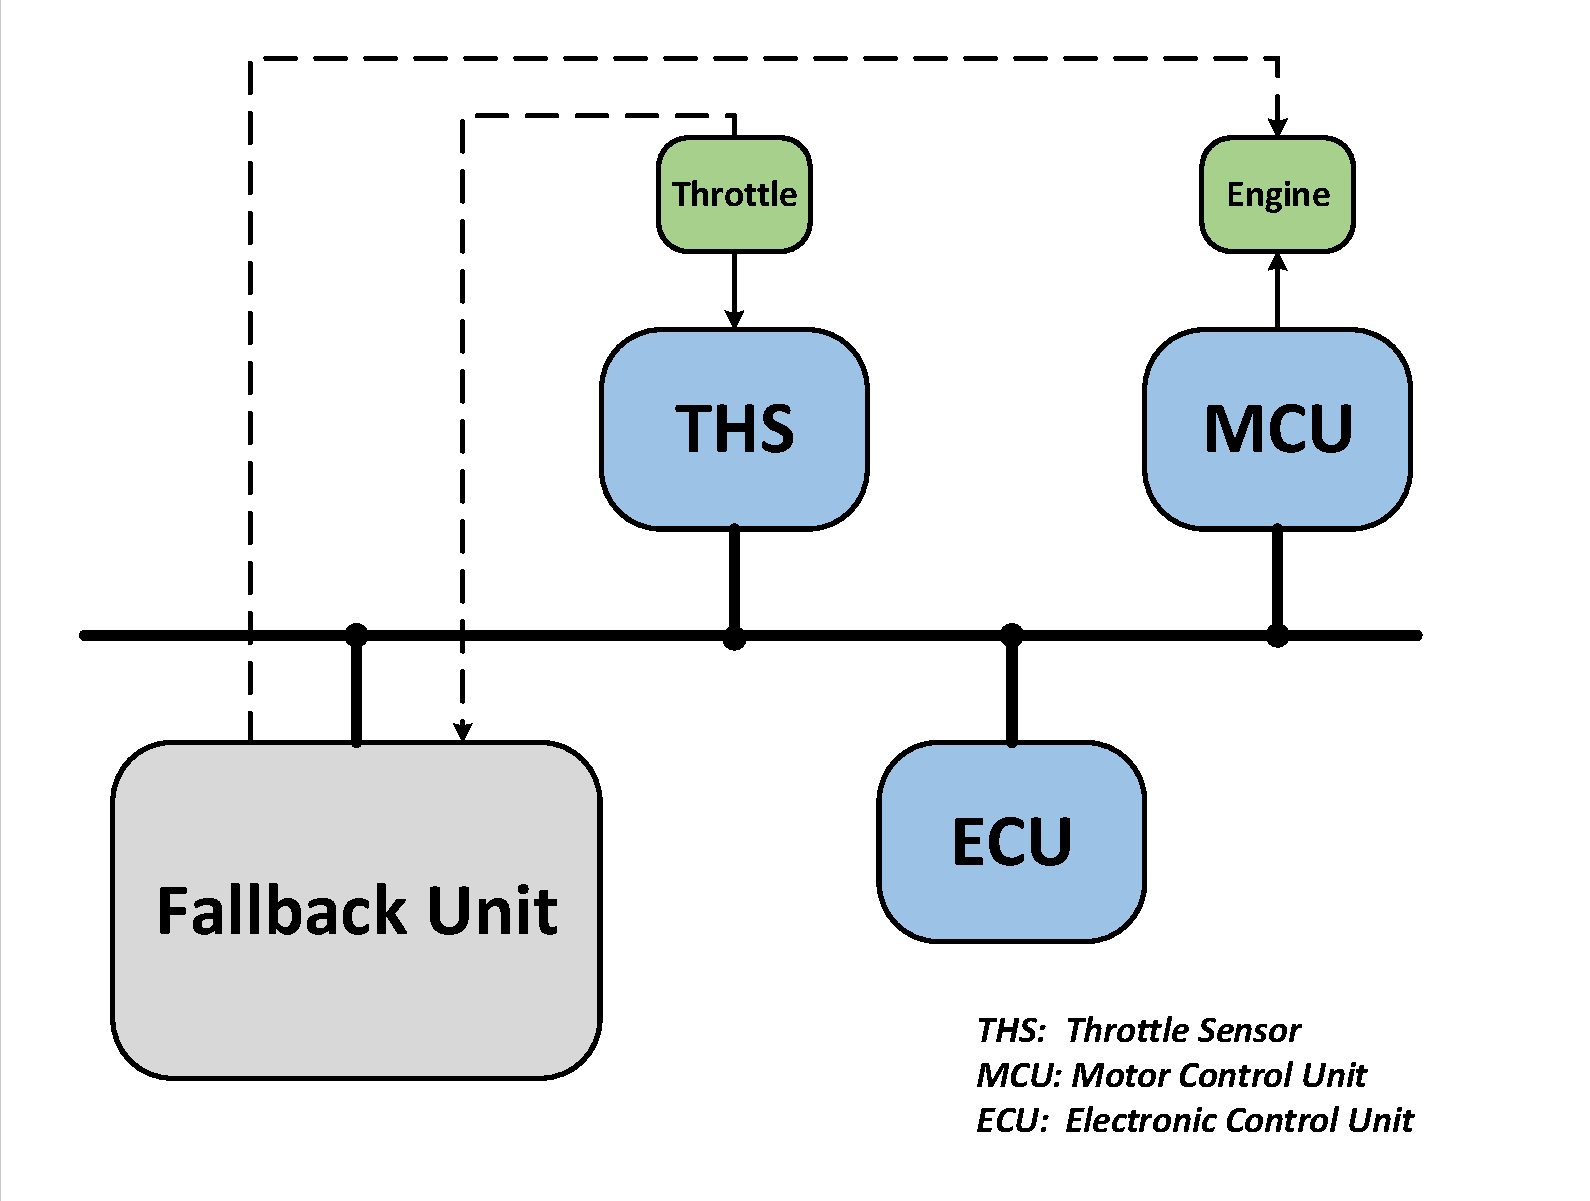
\includegraphics[width=0.75\textwidth]{figures/basic_design.pdf}
    \caption{Basic concept for Failsafe ECU}\label{fig:basicDesign}
\end{figure}

The realized scenario reads a throttle position and controls an engine after some data conversion. The \gls{ECU} is responsible for gathering the throttle position data, measured and provided by the \gls{THS}. After the \gls{ECU} converts the throttle position data into engine control data, it forwards these data to the \gls{MCU}, which is responsible for controlling the engine. A fourth unit acts as a fallback unit in case of a failure of one of the regular control units. This fallback unit is realized by using \gls{PR} in an \gls{FPGA}. Figure \ref{fig:sequenceNormalOp} displays a sequence diagram assuming normal operation. In this case, the fallback unit doesn't have to perform any active functionality, it just has to passively monitor the data transfer on the communication link to detect possible errors.

\begin{figure}[h!]
    \centering
    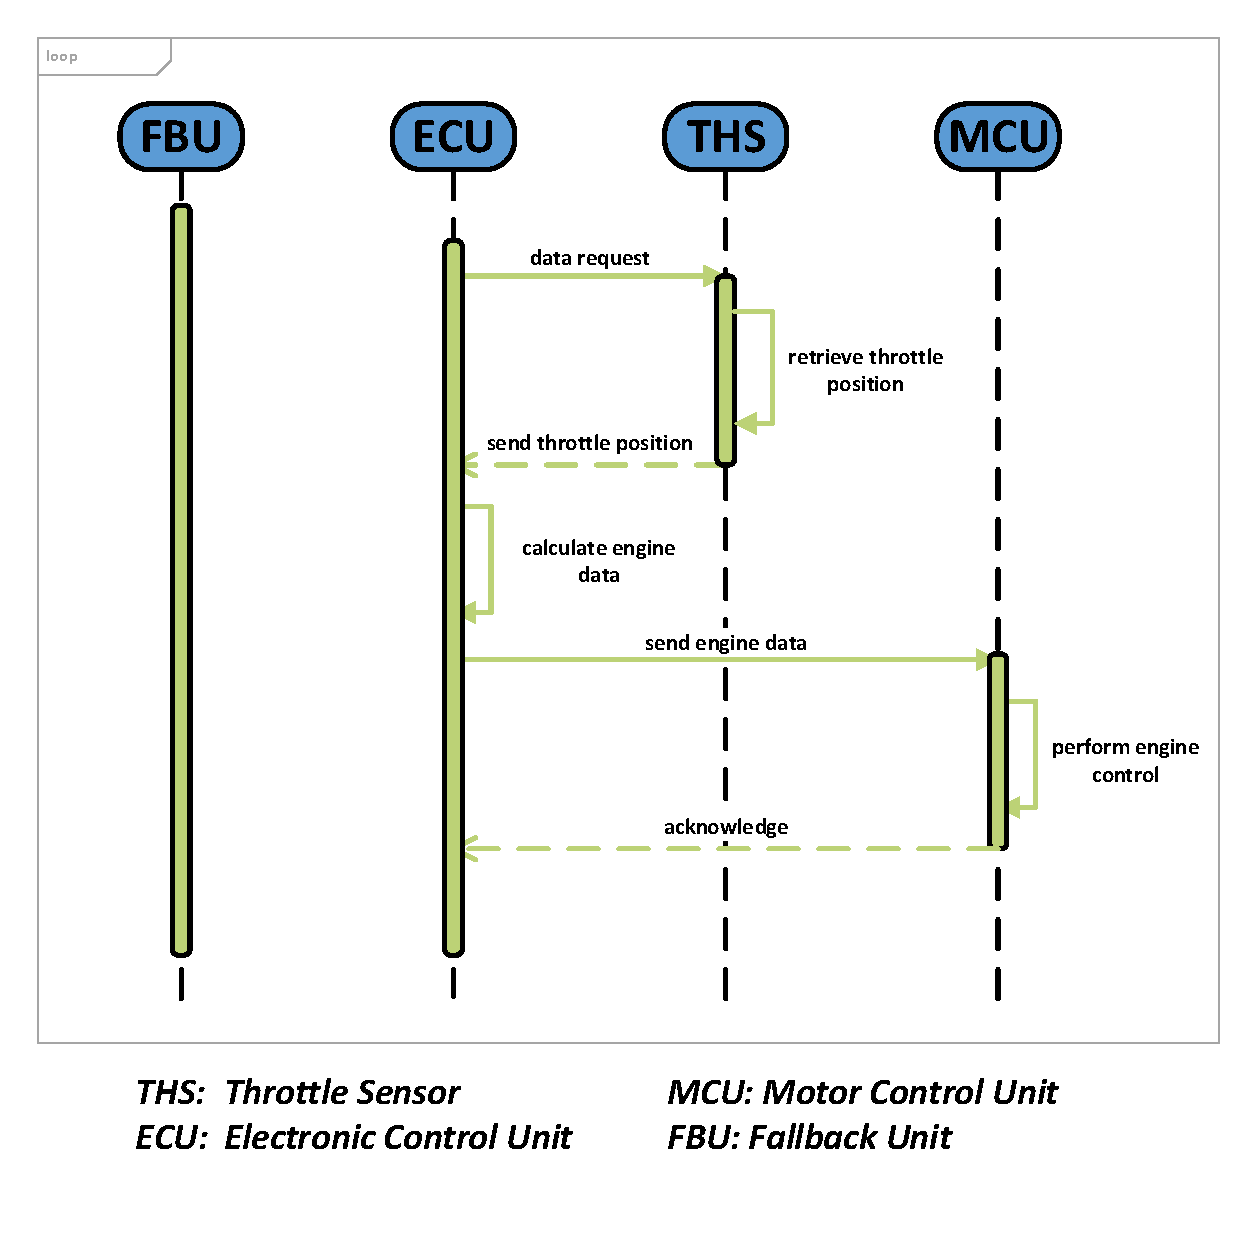
\includegraphics[width=\textwidth]{figures/sequence_normal_op.pdf}
    \caption{Sequence diagram for normal operation}\label{fig:sequenceNormalOp}
\end{figure}

The fallback unit has to monitor all transferred data on the bus and detect any failures (e.g. timeout, error flags, ...). 
Once an error is detected, a certain partial reconfiguration is triggered by the bus monitor module, which is part of the fallback unit. 
After the reconfiguration is finished, the fallback unit completely takes over the functionality of the faulty component. 
Due to the fail silent assumption, the faulty device will not affect the behaviour of the system. 
Figure \ref{fig:sequenceMCUFailure} shows a sequence diagram including a faulty \gls{MCU}. 
The bus monitor detects that the \gls{MCU} is running into a timeout and triggers a \gls{PR} to take over its functionality. 
After finishing the reconfiguration, normal operation takes over again (see figure \ref{fig:sequenceNormalOp}), but the fallback unit serves as \gls{MCU} now.

\begin{figure}[h!]
    \centering
    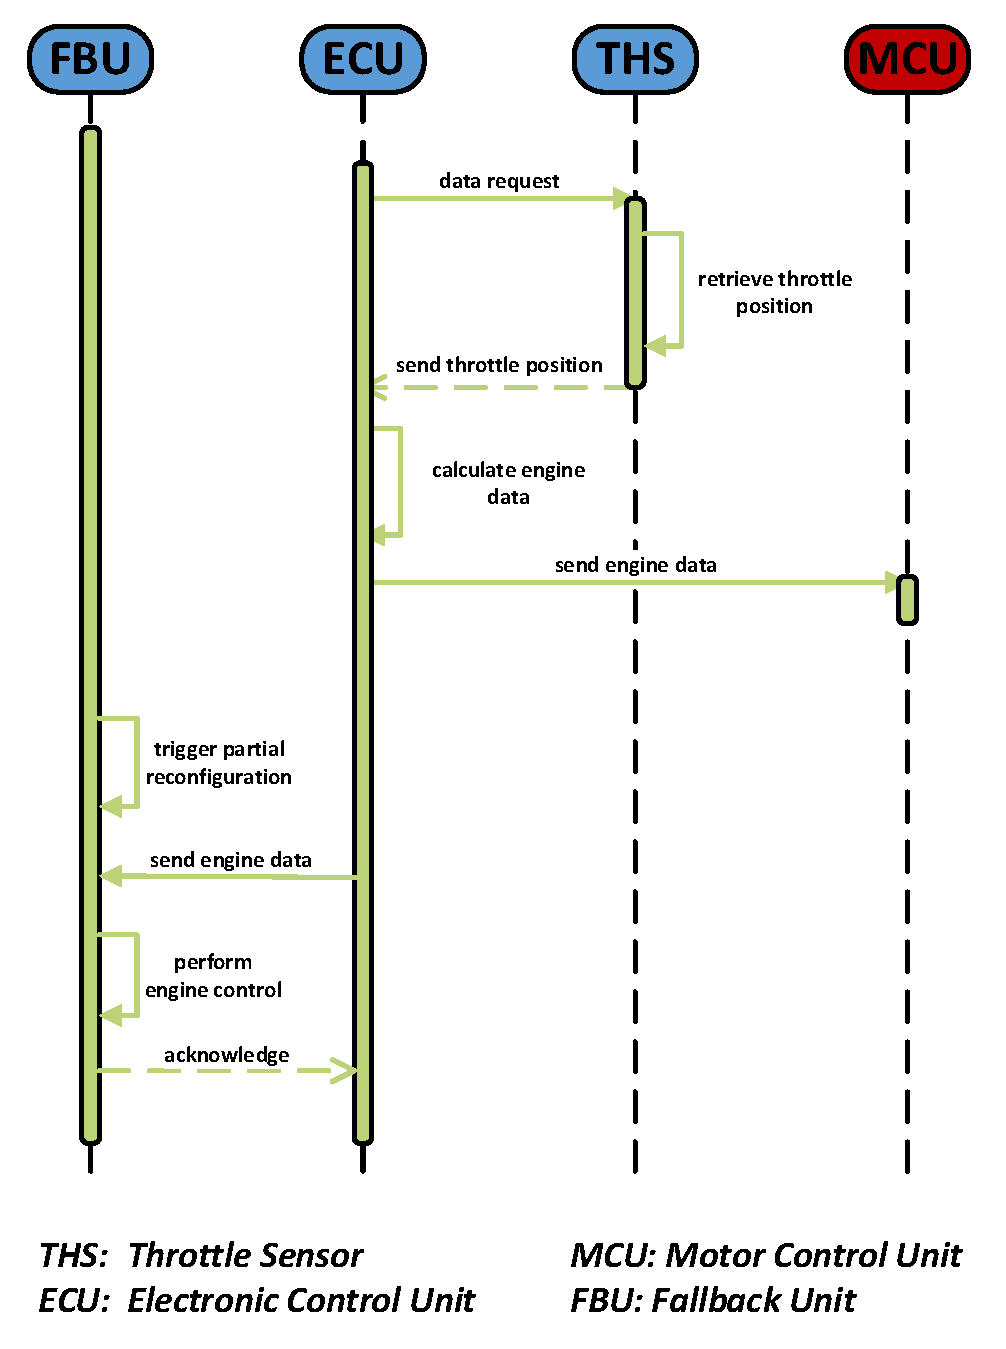
\includegraphics[width=\textwidth]{figures/sequence_mcu_fail.pdf}
    \caption{Sequence diagram for \gls{MCU} failure}\label{fig:sequenceMCUFailure}
\end{figure}

\section{Required tools, \glspl{IP} and packages}
TODO: licenses
\begin{itemize}
    \item Vivado 2018.3
    \item Vivado 2018.2
    \item uVision 5 (Windows only)
    \item ARM Keil (Windows only)
    \item ARM Cortex M1 IP for Vivado
    \item UART IP by Martin Mosbeck
    \item ARM Mbed OS
\end{itemize}

\section{Cortex M1 / M3}

Description of the setup of Cortex M1 and Cortex M3 Cores. \cite{arm_arm_2018} \cite{arm_cortex-m1_nodate}

\subsection{Usage of the Keil Toolchain}

Link to tutorial enough? Maybe most basic steps (e.g. adaption of arty project for our needs). \cite{noauthor_getting_nodate}

\subsection{Usage of Cortex M1 in Vivado}

Only global implementation / synthesis runs are permitted to obtain a working bitstream.
If OOC (Out of Context) runs are used, everything except for the Cortex M1 will work fine. 
The Cortex M1 will enter a hard-fault state which does not allow recovery. 
This is indicated by a high bit on the \textit{Lockup} port of the processor.

Also trivial, follow tutorial that is provided on ARM Website and adapt to own needs.

\subsubsection{Code via Memory Initialization File}

File is bound to synthesis process, how to change it...

\subsection{How to mbed OS}

How was the Cortex M1 Project adapted to support the Mbed OS?
What is gained through the usage of mbed OS?

\subsection{Implemented Functionality on the Cortex M1}

How are the UART and IIC peripherals supported in the source code, which libraries are used, interrupt based or not, performance?

Show highlights of the code?

\section{Bus and Peripherals}

\subsection{Used Peripherals}

What Peripherals were used (Cortex M1/M3 Boards, which ones).

How to program / use them (only brief).

How are they connected to the Bus?

IIC and UART here or in next section.

\subsection{Bus}

How is it set up?

Made assumptions?

Document used / invented protocol.


\chapter{Partial Reconfiguration}
This section reasons about design choices and encountered obstacles during the development process.

\section{Limitations imposed by partial reconfiguration}
\gls{PR} does impose some limitations on the design process, a brief description of the encountered limitations and how they were handled is given in the following.

\subsection{No block diagram support}
The \gls{PR} workflow as implemented by Xilinx in Vivado does not allow the \gls{RP} to be present in a block diagram.
Only hdl files are eligible for the \gls{PR} process.

To solve this problem without the loss of comfort that is provided by the usage of block diagrams (mainly the connection of different signals between modules) we decided to transfer our Cortex Module into an \gls{IP}-Package.
This \gls{IP}-Package can then be instantiated as a \gls{RTL} module alongside an existing block diagram.
Only the signal connections between the \gls{IP} and the block diagram have to be declared manually then.

\begin{figure}[ht]
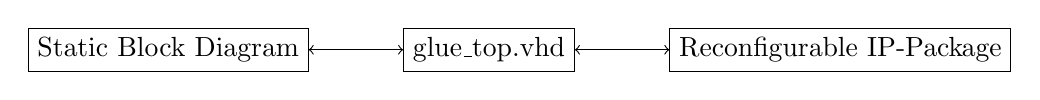
\begin{tikzpicture}[
    node distance = 0mm and 12mm,% for distance between nodes
       box/.style = {draw, very thick, minimum width=5em}% nodes style
    ]
    \node (n1) [draw] {Static Block Diagram};
    \node (n2) [draw, below right=of n1.north east] {glue\_top.vhd};
    \node (n3) [draw, below right=of n2.north east] {Reconfigurable IP-Package};
    \draw[<->] (n1) edge (n2);
    \draw[<->] (n2) edge (n3);
\end{tikzpicture}
\caption{Enable \gls{PR} by the separation of the block diagram and the \gls{RP}}\label{fig:blockDiagramGlue}
\end{figure}

Due to this, the originally planned AXI-Bus interface for the \gls{RP} needs to be connected manually. 
This has proven to be very error-prone in earlier evaluation steps and was then replaced by an interface that only exposed required signals.
An AXI-Bus interface may very well work though, as it probably failed due to other, unrelated errors.

\subsection{Global synthesis / implementation runs are mandatory}
\gls{PR} works with global synthesis and implementation runs only.
This imposes restrictions on the naming of files within packages. 
While \gls{OOC} runs allow the same instance names for different IPs a global run requires distinct file and instance names for everything that is included in the project.

Global synthesis and implementation runs are also necessary to include the memory initialization file for the Cortex processor. 

\subsection{\gls{PCAP} / \gls{ICAP} on the Zynq-7000}
As the Zynq-7000 was used for the prototyping process our first choice was the usage of the \gls{PCAP} for writing partial bitstreams to the \gls{FPGA} as it is the most straight forward (and well documented) way for this platform.

Due to design considerations (scaling well for production vs fast prototyping) a switch to using the \gls{ICAP} was made.
For this, the \gls{PCAP} needs to be actively deactivated after the boot of the processing system (\cite{zynq_7000_technical_manual}, page 218).

\subsection{\gls{ICAP} primitive instantiation}
Instantiation of the \gls{ICAP} as a hardware primitive in VHDL is documented in the 7series libraries guide (\cite{7series_libraries_guide}, page 178).
For completeness sake, the component definition is listed below as it does not exist directly in the documentation.
The comments the generic parameters that were used in this project.
\lstset{language=vhdl}
\begin{lstlisting}
component ICAPE2 is
generic (
    DEVICE_ID   : std_logic_vector(31 downto 0); -- X"23727093" 
    ICAP_WIDTH  : string; --"X32"
    SIM_CFG_FILE_NAME 	: string -- "None"
);   
port (
    O 		: out std_logic_vector(31 downto 0);
    CLK 	: in std_logic;
    CSIB 	: in std_logic;
    I 		: in std_logic_vector(31 downto 0);
    RDWRB 	: inout std_logic
);
end component ICAPE2;
\end{lstlisting}
\subsection{Read from SD-Card}
The SD-Card was used to provide a bootable image with the default configuration and all partial bitstreams.
Reads from the SD-Card may fail, resulting in a non-functioning or only partially functioning system.
The following steps should be performed to trouble-shoot the problem. 
\begin{itemize}
    \item If the system is working in its original configuration and only fails the partial reconfiguration, the file names of the bitstreams should be checked. Only a maximum of 8 characters (+3 for the extension) for the file name are permitted by default. 
    \item Slow (e.g. overwriting everything with zeros) reformat of the SD-Card may be tried.
    \item Smaller SD-Card should be tried.
\end{itemize}
\section{Integration Overview}
Due to our problems with the AXI-Bus it was decided to put all relevant peripheral communication into the \gls{RP}.
This eliminates the need of implementing an AXI-Interface at the cost of an increased size of the \gls{RP}.

The following modules are included in the \gls{RP}:
\begin{itemize}
    \item  AXI-GPIO
    \item  AXI-UartLite
    \item  Cortex M1
\end{itemize}

\begin{figure}[ht]
    \centering
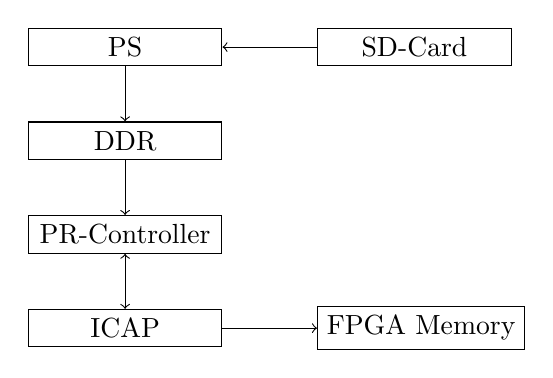
\begin{tikzpicture}[
    node distance = 7mm and 12mm,% for distance between nodes
       box/.style = {draw, minimum width=7em}% nodes style
    ]
    \node (n1) [box] {PS};
    \node (SD) [box, right=of n1.east] {SD-Card};
    \node (n2) [box, below =of n1.south] {DDR};
    \node (n3) [box, below =of n2.south] {PR-Controller};
    \node (n4) [box, below =of n3.south] {ICAP};
    \node (n5) [box, right =of n4.east] {FPGA Memory};
    \draw[->] (n1) edge (n2);
    \draw[->] (n2) edge (n3);
    \draw[<-] (n1) edge (SD);
    \draw[<->] (n3) edge (n4);
    \draw[->] (n4) edge (n5);
\end{tikzpicture}
\caption{Data path for loading a partial bitstream}\label{fig:prIntegration}
\end{figure}
\cite{xilinx_vivado_2018-1}, \cite{xilinx_vivado_2018}
Usage of \gls{ICAP}.
How is the Zynq still used - Loading images and binary blobs from sd card into DDR.
What is partially reconfigured - Cortex, uart, IIC.
Why not use AXI?
\subsection{Packaged IP}
The \gls{PR} IP was packaged according to the guide in \cite{xilinx_ug1118-vivado-creating-packaging-custom-ip.pdf_nodate}.
To avoid naming conflicts, all block designs of the different IPs need to be named differently before this process.
\subsection{Loading the \gls{PR} module}
The module is loaded through the \gls{PR}-Controller IP that is provided by Vivado. 
This module is connected via the AXI memory interface and loads the partial bitstream from DDR.
At start-up, the partial bitstreams are loaded form the SD-Card into the DDR through the Zynq \gls{PS} as it already needs to be used for the deactivation of the \gls{PCAP}.
Figure \ref{fig:prIntegration} shows how the different modules and memory entities are related to each other.
%\section{Organization}

\subsection{Assigned Sub-Tasks}
 \subsubsection{Cortex M1} 
 Evaluation of the provided Cortex-M1 from ARM and adaption of the provided toolchain to our needs. 

 Creation of a working stand-alone example, creation and integration of working IP-Packages for the Cortex-M1.

 Provision of partial reconfiguration eligible IP-Packages.
 \subsubsection{Partial Reconfiguration}
 Evaluation of the partial reconfiguration flow in Vivado (project vs. script based).

 Determination of restrictions that come with partial reconfiguration e.g. less flexible and limited use of clock spines within the pr region, no operations on clocks within the pr region, constant interface over all implementations, placement / alignment restrictions, naming conventions and conflicts for custom IP-Packages, binding usage of .vhd files instead of block diagrams with regards to pr modules. 

 Evaluation with Microblaze processors, as Cortex M1 is only available from the start of November 2018.

 Generation of a Bootable Image that includes the partial reconfiguration bitstreams in a binary format.

 Modification of the Zynq processing system on the Zedboard to allow for the usage of the ICAP instead of the PCAP, loading the partial bitstreams into DDR memory from the SD-Card.

 Evaluation of the pr-controller and the available trigger sources / types.
 \subsubsection{Bus Design}
 Protocol, Standard, Implementation on FPGA / Cortex.
 \subsubsection{Hardware}
 Evaluation of hardware types (e.g. Nucleo Boards), possible connection to the Zedboard, CAN-Driver boards. 
\subsection{Estimated Contribution}
Contribution to the project was roughly the same for each group member.
Table \ref{tbl:AssignedTasks} shows the tasks and how they were assigned to the different team members.
    \begin{table}
        \centering
\begin{tabular}{ l | c c c c c}
 Task & Hirtenlehner & Schieber & Schober & Schorn\\ 
 \hline
Cortex M1       & X & X & X &   \\
Partial Reconf. &   & X &   &   \\
Bus Design      &   &   &   & X \\
Hardware        & X &   &   & X \\
Mbed OS         & X &   &   & X \\
\end{tabular}
\caption{Distribution of tasks within the group}
\label{tbl:AssignedTasks}
\end{table}
\chapter{Results}
\section{Conclusion}
This work has explored the possibility of using partial reconfiguration in \glspl{FPGA} to provide efficient redundancy in an automotive system.
Instead of providing a redundant hardware entity for every critical module, one single \gls{FPGA} provides dynamic redundancy for each of these modules.
To avoid over-commitment with regards to resource usage (space and power) partial reconfiguration is used.
By using the newly available Cortex M1 IPs, a streamlined software development process is possible. 
The same software can be executed on the cores in the \gls{FPGA} as well as on the actual hardware with minimal adaptions in the build-process.
This reduces the amount of testing and tool-chain adaptions that need to be performed.
We demonstrated these concepts on the Zynq-7000 and with three Cortex M1 \glspl{CPU} that were connected with a bus.

\subsection{Future Work}
Based on this work a more heterogeneous set of critical hardware could be provided with redundancy. 
A good first step would be to include the Cortex M3 CPU that couldn't be included in this project due to time constraints.
The bus monitor could be extended with a more sophisticated fault detection algorithm, which could also mean to employ a more sophisticated bus protocol.
Measurements with regards to the system performance (e.g. time to reconfigure, time to detect fault, time to mitigate fault, power usage ...) should be considered also.  

\bibliographystyle{IEEEtran}
\bibliography{IEEEabrv,SoCLabor}

\end{document}

